\chapter{Thompson Sampling Based Algorithms for Exploration in Reinforcement Learning}\label{C:ts}
A desirable property of sampling strategies is to have theoretical proves of their efficiency in terms of the number of collected samples. Among others, the principle of \gls{ofu}~\cite{lai1985asymptotically} has been well studied in literature where large evidence of its efficiency is given~\cite{jaksch2010near, kakade2003sample, kearns2002near}. \gls{ofu} states that actions with statistically uncertain values are to be favored (e.g., through an exploration bonus) in the action-selection process compared to the more certain ones in order to improve the knowledge of the environment. This optimistic sampling strategy speedups the learning of the action values and efficiently exploits them as the uncertainty about the environment is reduced, and thus the effect of optimism lessens. This sampling strategy has been firstly used in the context of \glspl{mab} and is known as \gls{ts}~\cite{thompson1933likelihood}. The idea of \gls{ts} is to randomly choose an arm (i.e., an action) to be drawn according to its probability of being the optimal one. Interestingly, several recent works based on \gls{ts} and showing promising results have been proposed~\cite{chapelle2011empirical, granmo2010solving, may2011simulation, scott2010modern}. The use of \gls{ts} in \gls{rl} seems quite straightforward considering the actions of the \gls{mdp} as the arms of the \glspl{mab}; nevertheless, the presence of multiple states and dynamic transitions among them makes the estimation of uncertainty a challenging problem in this setting. Indeed, the estimation of the action-value uncertainty in each state of the \gls{mdp} is the critical part of a sampling strategy based on optimism (e.g. \gls{ts}) since computational and sample efficiency have to be taken into account in order to make optimism-based strategies feasible.

One widely used approach to model uncertainty is discussed in the literature about \textit{intrinsically motivated} \gls{rl}~\cite{chentanez2005intrinsically, schmidhuber1991possibility} where the number of visits to a state is inversely related to the uncertainty of its value and is used to generate an intrinsic reward that guides the exploration~\cite{bellemare2016unifying, tang2017exploration}. Other techniques to represent the interest of a state have been proposed, for instance, relying on the amount of knowledge a deep learning model has of a specific state~\cite{pathak2017curiosity} or considering the representativeness of a state w.r.t. the \gls{mdp}~\cite{bonarini2006self}. Despite their effectiveness, these methods become more inefficient w.r.t. the dimensionality of the problem because of the complexity of representing the intrinsic reward.

Our work takes inspiration from the Bayesian \gls{rl} framework where a probability distribution is used to model the uncertainty over action value functions in each state. One of the first works following this approach is Bayesian Q-Learning~\cite{dearden1998bayesian} which proposes to estimate the action values initializing them with a prior distribution and updating their posterior distribution each time a new sample is collected from the \gls{mdp}. Our work is motivated by the fact that in the Bayesian approach the variance of the distribution can be used as a measure of the uncertainty of the action allowing to pursue \gls{ofu} using \gls{ts}.

We present several methodologies to efficiently compute the uncertainty of action values in online \gls{rl} problems and to use \gls{ts} strategy. We propose two main techniques to accomplish these tasks, one of them suitable for low-dimensional problems and the other one specifically proposed for high-dimensional ones. We discuss the properties of these methods and consider \glspl{mdp} where the exploration is a critical aspect to empirically show how \gls{ts} can outperform other sampling strategies in terms of performance and sample-complexity independently from the dimensionality of the problem. 

\section{Related work}
The convergence of many \gls{rl} algorithms is guaranteed when the exploration policy allows visiting each state for an infinite number of times. Common sampling strategies like $\varepsilon$-greedy or Boltzmann guarantee the convergence property, but they can suffer from unfeasible learning time. For this reason, finite-time bounds for convergence are a desirable property of exploration policies to understand the theoretical guarantees about the feasibility of a learning algorithm based on them. The problem of finding finite-time bounds is addressed in several works that propose nearly-optimal sampling strategies with polynomial bounds for convergence time. Most of these works are based on enhancing the probability of choosing actions that allow the agent to explore, i.e. to collect state-action samples never (or not sufficiently) seen before, thus pursuing the principle of \gls{ofu}. Among them, UCRL~\cite{auer2007logarithmic} and UCRL2~\cite{jaksch2010near} guarantee logarithmic regret bounds applying the idea of using an upper bound on the estimate of action values and exploring with an optimistic policy, as done in the UCB1~\cite{auer2002finite} algorithm used in MABs. A similar approach is proposed in Delayed Q-Learning~\cite{strehl2006pac} where the action values are initialized to high values, and an optimistic policy is used. Model-based methodologies based on the same reasonings have also been proposed such as, among others, the E$^3$~\cite{kearns2002near} algorithm and the later R-MAX~\cite{brafman2002r} algorithm. However, despite the desirable theoretical properties, these algorithms usually do not work well in practice, and most importantly they do not scale well w.r.t. the dimensionality of the problem.

A different approach to pursue \gls{ofu} is to use a Bayesian framework. The literature on Bayesian RL offers a large number of works that can be split into model-based and value-based ones. The model-based ones propose to start from a prior distribution over MDPs and compute the respective posterior distribution as newer samples are collected from the \gls{mdp}~\cite{dearden1999model, kolter2009near}. Following this approach, the \gls{psrl}~\cite{strens2000bayesian} method consists in maintaining a probability distribution over \glspl{mdp}, generating a hypothesis from it at the beginning of each episode and running the greedy policy w.r.t. the generated \gls{mdp}. This method guarantees convergence to the optimal policy for a stationary process with discrete states. An extension of this work which shows a better upper bound on expected regret for \gls{psrl} is presented in~\cite{osband2013more}. Unfortunately, these algorithms do not scale well w.r.t. the complexity of the \gls{mdp} since building the model of them can be impractical.
Value-based methods can overcome the drawbacks of model-based ones using randomized value functions sampled by probability distributions. The first algorithm based on a Bayesian approach is Bayesian Q-Learning~\cite{dearden1998bayesian}. This algorithm starts from a prior over action values, instead of \glspl{mdp}, updates the posterior distribution of these action values as new samples are collected from the \gls{mdp} and run an optimistic policy, such as \gls{ts}, w.r.t. them. The recent Weighted Q-Learning~\cite{deramo2016estimating} algorithm follows a similar approach, but it simplifies the cumbersome action values update of Bayesian Q-Learning starting by the assumption that the probability distribution of action values can be approximated as a normal distribution according to the central limit theorem. Then, the variance of the normal distribution is used as the measure of uncertainty over the action values, and \gls{ts} can be used. 
Other recent works that follow a value-based approach to the problem are \gls{rlsvi}~\cite{osband2016generalization} and its extension to the \gls{drl} setting \gls{bdqn}~\cite{osband2017deep}, which we consider later in this work.

\section{Thompson Sampling in value-based Reinforcement Learning}\label{S:tsrl}
We want to use gls{ts} as a sampling strategy in \gls{rl} problems, i.e. to sample an action from each state according to its probability of being the optimal one.
We consider an \gls{mdp} with discrete actions and an unknown probability distribution associated with the action value function $Q(s,a), \forall s \in \mathcal{S}, a \in \mathcal{A}$. Let $f_i:\mathbb{R} \rightarrow \mathbb{R}$ be the \gls{pdf} and $F_i:\mathbb{R} \rightarrow \mathbb{R}$ be the \gls{cdf} of the action value function $Q_i(s) = Q(s, a_i), \forall s \in \mathcal{S}$, and $\mu_i(s)$ and $\sigma^2_i(s)$ be respectively the mean and the variance of these distributions. The \gls{pdf} and \gls{cdf} of the approximated action value function $\tilde{Q}_i(s)$ are denoted, respectively, as $\tilde{f}_i^s$ and $\tilde{F}_i^s$ with mean $\tilde{\mu}_i(s)$ and variance $\tilde{\sigma}_i^2(s)$. Thus, the probability of each action $a_i$ to be the optimal one in a given state $s$ can be computed as:

\begin{equation}\label{E:max_prob}
 P\left(\tilde{Q}_i(s) = \max_j \tilde{Q}_j(s)\right) = P\left(\tilde{Q}_i(s) \geq \tilde{Q}_j(s), \forall j \neq i\right) = \int^{+\infty}_{-\infty} \tilde{f}_i^s(x) \prod_{j \neq i} \tilde{F}_j^s(x) dx.
\end{equation}

Using the probabilities $P\left(\tilde{Q}_i(s) = \max_j \tilde{Q}_j(s)\right)$ computed in Equation~\ref{E:max_prob}, \gls{ts}\footnote{Sometimes, in the \gls{rl} literature, sampling strategies equivalent to \gls{ts} are named in a different way (e.g. Q-value sampling~\cite{dearden1998bayesian}).} can be done sampling an action from the discrete density function resulting from them. Since we are only interested in selecting the action, we can avoid the expensive computation of the integral by merely sampling a value from each $\tilde{f}_i$ and selecting the action corresponding to the sampled maximum action value without loss of precision.

The approximation of the unknown \glspl{pdf} and \glspl{cdf} is done relying on the \gls{clt}, as proposed in~\cite{d2016estimating}, which states that as the number of samples $N_i^s$ retrieved from the sampling distribution $\tilde{f}_i^s$ increases, $\tilde{f}_i^s$ approaches the normal distribution independently from the real distribution $f_i^s$, i.e., $\tilde{f}_i^s \approx \mathcal{N}\left(\tilde{\mu}_i(s), \frac{\tilde{\sigma}^2_i(s)}{N_i^s}\right)$, where $\tilde{\mu}_i(s)$ is the sample mean and $\tilde{\sigma}^2_i(s)$ is the sample variance. 

\section{Efficient uncertainty estimation}\label{S:uncertainty}
The use of \gls{clt} explained in Section~\ref{S:tsrl} allows representing the uncertainty of $\tilde{Q}_i(s) = \tilde{\mu}_i(s)$ with the sample variance $\frac{\tilde{\sigma}^2_i(s)}{N_i^s}$. The remaining problem is the computation of $\tilde{\sigma}^2_i(s)$ in an efficient and scalable way w.r.t. the complexity of the \gls{mdp}. We propose two main methods to deal with this problem. The former consists in updating the uncertainty in an online fashion and is specifically proposed to be used in discrete \glspl{mdp}; nevertheless, we discuss its extension to continuous state spaces, that is however only practical for low-dimensional ones. The latter exploits the bootstrapping method to compute the variance, thus being more suitable for dealing with high-dimensional \glspl{mdp} efficiently and, moreover, it does not need a Gaussian approximation of the action value functions.

\subsection{Online estimation}
Firstly we introduce the standard procedure to incrementally compute the update of the mean and the exponentially weighted update of the variance (Algorithm~\ref{A:var_1}). An alternative method, which is more suitable for computational reasons but is slightly more biased than the previous one, is to estimate the variance as the difference between the second order momentum and the square of the first order one (Algorithm~\ref{A:var_2}).
\begin{algorithm}[t]
 \caption{Standard mean and variance update}
 \begin{algorithmic}[1]\label{A:var_1}
  \STATE \textbf{Inputs:} current mean $\overline{X}$, current variance $S^2$, new sample $x$, learning rate $\alpha$
  \STATE $\Delta_{\overline{X}} \gets x - \overline{X}$
  \STATE $\overline{X} \gets \overline{X} + \alpha \Delta_{\overline{X}}$
  \STATE $S^2 \gets (1 - \alpha)(S^2 - \alpha \Delta_{\overline{X}}^2)$
 \end{algorithmic}
\end{algorithm}
\begin{algorithm}[t]
 \caption{Mean and variance update using momentums}
 \begin{algorithmic}[1]\label{A:var_2}
  \STATE \textbf{Inputs:} current mean $\overline{X}$ , current squared mean $\overline{X^2}$, current variance $S^2$, new sample $x$, learning rate $\alpha$
  \STATE $\Delta_{\overline{X}} \gets x - \overline{X}$
  \STATE $\Delta_{\overline{X^2}} \gets x^2 - \overline{X^2}$
  \STATE $\overline{X} \gets \overline{X} + \alpha \Delta_{\overline{X}}$
  \STATE $\overline{X^2} \gets \overline{X^2} + \alpha \Delta_{\overline{X^2}}$
  \STATE $S^2 \gets \overline{X^2} - \overline{X}^2$
 \end{algorithmic}
\end{algorithm}
The previously described procedures can be easily integrated into the update rule of many RL algorithms; in the following sections, we use SARSA as a reference case. Since we are interested in the variance of the estimator, we have to normalize the variance of the process $\sigma^2_{process}$ by the number of effective samples that is limited by the learning rate. Let $\alpha_i$ be the learning rate at the $i$-th update, we compute the effective sample size as:
\begin{equation}
 n_{eff} = \frac{(\sum_{i=1}^n \omega_i)^2}{\sum_{i=1}^n \omega_i^2},
\end{equation}
where $\omega_i = \alpha_i\prod_{k=i+1}^K{(1-\alpha_k)}$ is the weight of the $i$-th sample and $K$ is the number of collected samples.
Then, we derive the update rule for SARSA with variance estimation, as shown in Algorithm~\ref{A:sarsa_var}.
\begin{algorithm}[t]
\caption{SARSA with online variance update}
\begin{algorithmic}[1]\label{A:sarsa_var}
  \STATE \textbf{Inputs:} state $s$, action $a$, reward $r$, next state $s'$, learning rate $\alpha$, discount factor $\gamma$
  \STATE $a' \gets \pi(s')$
  \STATE $\omega (s,a) \gets (1 - \alpha) \omega (s,a) + \alpha$
  \STATE $\omega^2 (s,a) \gets (1 - \alpha)^2 \omega^2 (s,a) + \alpha ^2$
  \STATE $n_{eff} \gets \frac{\omega(s,a)^2}{\omega^2(s,a)} $
  \STATE $target \gets r + \gamma Q(s',a')$
  \STATE $\sigma^2_{process}(s,a) \gets (1 - \alpha)\left(\sigma^2_{process}(s,a) + \alpha (target - Q(s,a))^2\right)$
  \STATE $\sigma^2_{estimator}(s,a) \gets \frac{\sigma ^2_{process}(s,a)}{n_{eff}}$
  \STATE $Q(s,a) \gets Q(s,a) + \alpha \left(target - Q(s,a)\right)$
\end{algorithmic}
\end{algorithm}
\begin{algorithm}
\caption{SARSA with online variance update and Hoeffding upper bound}
\begin{algorithmic}[1]\label{A:sarsa_hoeff}
  \STATE \textbf{Inputs:} state $s$, action $a$, reward $r$, next state $s'$, learning rate $\alpha$, discount factor $\gamma$, 
  \STATE $a' \gets \pi(s')$
  \STATE $\text{Update } n_{eff}(s,a) \text{ as in Algorithm~\ref{A:sarsa_var}}$
  \STATE $target \gets r + \gamma Q(s',a')$
  \STATE $Q(s,a) \gets Q(s,a) + \alpha (target - Q(s,a))$
  \STATE $m_1(s,a) \gets Q(s.a)$
  \STATE $m_2(s,a) \gets m_2(s,a) + \alpha \left(target^2 - m_2(s,a)\right)$
  \STATE $\varepsilon_{m_1} = \sqrt{\frac{R_1^2\log{\frac{1}{\delta}}}{2n_{eff}}}$ 
  \STATE $\varepsilon_{m_2} = \sqrt{\frac{R_2^2\log{\frac{1}{\delta}}}{2n_{eff}}}$
  \STATE $\sigma^2_{process}(s,a) \gets \min(m_2(s,a) + \varepsilon_{m_2}, R_{2_{max}}) - \left(\max(m_1(s,a) + \varepsilon_{m_1}, R_{1_{min}})\right)^2$
  \STATE $\sigma^2_{estimator}(s,a) \gets \frac{\sigma ^2_{process}(s,a)}{n_{eff}}$
\end{algorithmic}
\end{algorithm}
In order to desirably boost exploration, the variance estimator $\sigma^2_{estimator}(s,a)$ can be replaced with an upper bound of it chosen among the ones provided in statistics.
\begin{enumerate}
\item  In line with the Gaussian approximation, we recall the confidence interval on variance provided by the $\chi^2$ distribution:
\begin{equation}
 \sigma^2_{upper bounded}(s,a) \gets \frac{(N - 1)\sigma^2_{estimator}(s,a)}{ \chi^2_{\frac{\beta}{2}, N - 1}},
\end{equation}
where $N = \lceil{n_{eff}}\rceil$ and $\beta$ is the significance level of the test. This upper bound may not be enough to induce enough exploration in \glspl{mdp} with a sparse reward function, especially at the beginning of the learning process when the action value function is initialized to zero.
\item Another upper bound is given by the Hoeffding bound~\cite{hoeffding1963probability}. Let $x_1, ... , x_n$ be independent and identically distributed bounded random variables such that $x_i$ falls in the interval $[a, b]$, then for any $\varepsilon > 0$:
\begin{equation}\label{E:hoeff}
 P( \overline{X} - E[\overline{X}]  > \varepsilon ) \leq e^{-\frac{2N \varepsilon^2}{(b-a)^2}} 
\end{equation}
where $\overline{X} = \frac{1}{N}\sum_{i=1}^N{x_i}$. From Equation~\ref{E:hoeff} we can derive the bound on the error relative to a probability $(1-\delta)$ for the inequality to hold:
\begin{equation}
 \varepsilon(N) = \sqrt{\frac{(b-a)^2\log{\frac{1}{\delta}}}{2N}}.
\end{equation}
From these considerations, we can derive the variance estimation method shown in Algorithm~\ref{A:sarsa_hoeff} where $R_1$ and $R_2$ are the ranges of possible values of, respectively, $m_1$ and $m_2$ and where the upper bound is computed as the difference between the upper bound of the second order momentum and the lower bound of the first order one. In practice this approach solves the problem of the initial lack of exploration, but since the range of the expected return is usually a large number, delays too much the exploitation phase. A way to overcome this issue, is to sum the variance with a term, similar to the Hoeffding bound, that uses a parameter which allows to tune the amount of exploration in the first stages of learning:
\begin{equation}
 \sigma^2_{upper bounded} \gets \sigma^2_{estimator} + \frac{c}{\sqrt{n_{eff}}}.
\end{equation}
\item The previous upper bound can be used in addition to the $\chi^2$ upper bound in order to boost the exploration when the number of samples is low and to have the benefits given by the $\chi^2$ upper bound during later stages of the learning process:
\begin{equation}
 \sigma^2_{upper bounded}[s,a] \gets \frac{(N - 1)\sigma^2_{estimator}[s,a]}{ \chi^2_{\frac{\beta}{2}, N - 1}} + \frac{c}{\sqrt{n_{eff}}}.
\end{equation}
\end{enumerate}
\begin{algorithm}[t]
\caption{SARSA with function approximation with variance update}
\begin{algorithmic}[1]\label{A:SARSA-apprx}
  \STATE \textbf{Inputs:} state $s$, action $a$, reward $r$, next state $s'$
  \STATE $a' \gets \pi(s')$
  \STATE $\text{Update } n_{eff}(s,a) \text{ as in Algorithm~\ref{A:sarsa_var}}$
  \STATE $Q_{target} \gets r + \gamma Q[s',a'; \theta]$
  \STATE $\Delta Q \gets Q_{target} - Q[s,a; \theta]$
  \STATE $\sigma^2_{process_{target}} \gets (1 - \alpha)\Delta Q^2$
  \STATE $\Delta \sigma^2_{process} \gets \sigma^2_{process_{target}} - \sigma^2_{process}[s,a; \theta']$
  \STATE $\theta \gets \theta + \alpha \Delta Q \nabla Q[s,a; \theta]$
  \STATE $\theta' \gets \theta' + \alpha \Delta \sigma^2_{process} \nabla \sigma^2_{process}[s,a; \theta']$
\end{algorithmic}
\end{algorithm}
The previous techniques cannot be applied in \glspl{mdp} with \textbf{continuous state spaces} since a tabular representation of the variance is not suitable. In these problems, the variance of the process can be approximated using an adaptation of the procedures in Algorithm~\ref{A:var_1} and Algorithm~\ref{A:var_2}. While the latter is immediate since it simply requires to estimate the second order momentum in addition to the first order one, the former is a bit less straightforward, and we show the procedure in Algorithm~\ref{A:SARSA-apprx}. In this case, the problem we are left with is the estimation of the effective sample size for each state-action tuple, but, when the state space is finite and has only a few dimensions, discretization is the most straightforward alternative. For instance, this can be done using tilings features or, in case of large input spaces (e.g. pixel frames of a game), using an autoencoder as hash-function~\cite{tang2017exploration}.

\subsection{Bootstrapping}
We propose \textit{bootstrapping} to compute the variance in \glspl{mdp} with high-dimensional continuous state space where the previous method, based on the discretization of the state space, would be inefficient. Bootstrapping consists in training different regressors of the target function with datasets obtained through sampling with replacement from the original dataset~\cite{doi:10.1162/089976600300015204}. The approximation of the variance of the estimate can be directly computed as the variance of the target function estimates provided by each regressor. To implement our idea, we consider the \gls{bdqn} algorithm~\cite{osband2017deep}, a variant of the famous \gls{dqn} algorithm~\cite{mnih2015human}, able to reach remarkable results in \gls{drl} problems. The main contribution of \gls{bdqn} is the introduction of a policy based on bootstrapping and inspired by posterior sampling~\cite{osband2013more} that, at the beginning of each episode, randomly samples one of the regressor in the ensemble and follows the greedy policy derived by it.

\paragraph{Thompson Sampling via Bootstrapping} We propose to use the framework provided by \gls{bdqn} and replace its exploration policy with \gls{ts}.\footnote{In their article, the authors of \gls{bdqn} discuss a variant of the proposed policy which they call Thompson \gls{dqn}. This simply modifies \gls{bdqn} sampling a head at each step instead of at the beginning of each episode. However we think this does not correspond to an appropriate application of \gls{ts} in this setting since the action values are not sampled from the distribution provided by the bootstrapped network.} Since the bootstrapped network provides a distribution over action value functions, we claim that \gls{ts} can be applied in this setting by picking, at each step and for each action, the action value from a randomly chosen head; then, executing the action whose action value is the highest among the sampled ones.
\gls{bdqn} consists in using an ensemble of $K \in \mathbb{N_+}$ action value function approximators. This ensemble can be created both using multiple neural networks, or splitting the output of only one neural network in multiple heads, each of which representing the $\tilde{Q}_k $ estimate of the real action value function $Q$. Bootstrapping is performed diversifying the heads with the random initializations of their weights and assigning a randomly generated binary mask $m_1, \dots, m_K \in [0,1]$ to each sample to indicate which head should be trained with it. Moreover, the update of \gls{ddqn}~\cite{van2016deep} is used in place of the standard \gls{dqn} update to avoid the overestimation issue. Finally, the exploration policy consists in sampling a head at the beginning of each episode and following the greedy policy induced by it. On the other hand, evaluation is performed by ensemble voting.

The application of \gls{ts} in \gls{bdqn} simply consists in changing its exploration policy. Algorithm~\ref{A:tsboot} shows the pseudocode of \gls{ts} via bootstrapping.
\begin{algorithm}
\caption{Bootstrapped DQN with Thompson Sampling}
\begin{algorithmic}[1]\label{A:tsboot}
  \STATE \textbf{Inputs:} action value function network $Q$ with $K$ outputs $Q_{k=1}^K$. Masking distribution $M$. Replay Buffer $B$ storing experience for training.
  \REPEAT
  \STATE Obtain state $s_t$ from the environment
  \STATE Sample action values $a_t^i$ from a randomly chosen head $Q_k$ for each action $i$
  \STATE Perform action $a_t$ which is the action $a_t^i$ with the largest value among the sampled ones, observe reward $r_t$ and reached state $s_{t+1}$
  \STATE Sample bootstrap mask $m_t \sim M$
  \STATE Add $(s_t, a_t, r_t, s_{t+1}, m_t)$ to replay buffer $B$
  \UNTIL End condition is satisfied
\end{algorithmic}
\end{algorithm}

\paragraph{Bootstrapped Q-Learning} We slightly modify \gls{bdqn} to adapt it for discrete \glspl{mdp}. We use a tabular approximation of the action value functions instead of using a deep neural network and update the action value functions using the Double Q-Learning update rule~\ref{S:mev_works}. To perform bootstrapping, the action value functions are initialized randomly and masking is used as in \gls{bdqn}.

\begin{figure}[t]
\begin{minipage}{.66\textwidth}
\begin{center}
  \subfigure[Online variance\label{F:taxi_online}]{\includegraphics[scale=.045]{img/comp.pdf}}
\end{center}
\end{minipage}
\begin{minipage}{.33\textwidth}
\begin{center}
  \subfigure[Taxi grid\label{F:taxi_grid}]{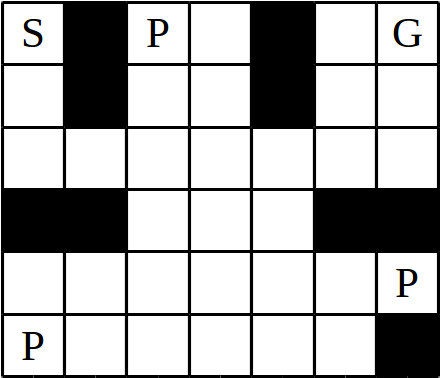
\includegraphics[scale=.25]{img/taxi.png}}
  \subfigure[Bootstrapped variance\label{F:taxi_boot}]{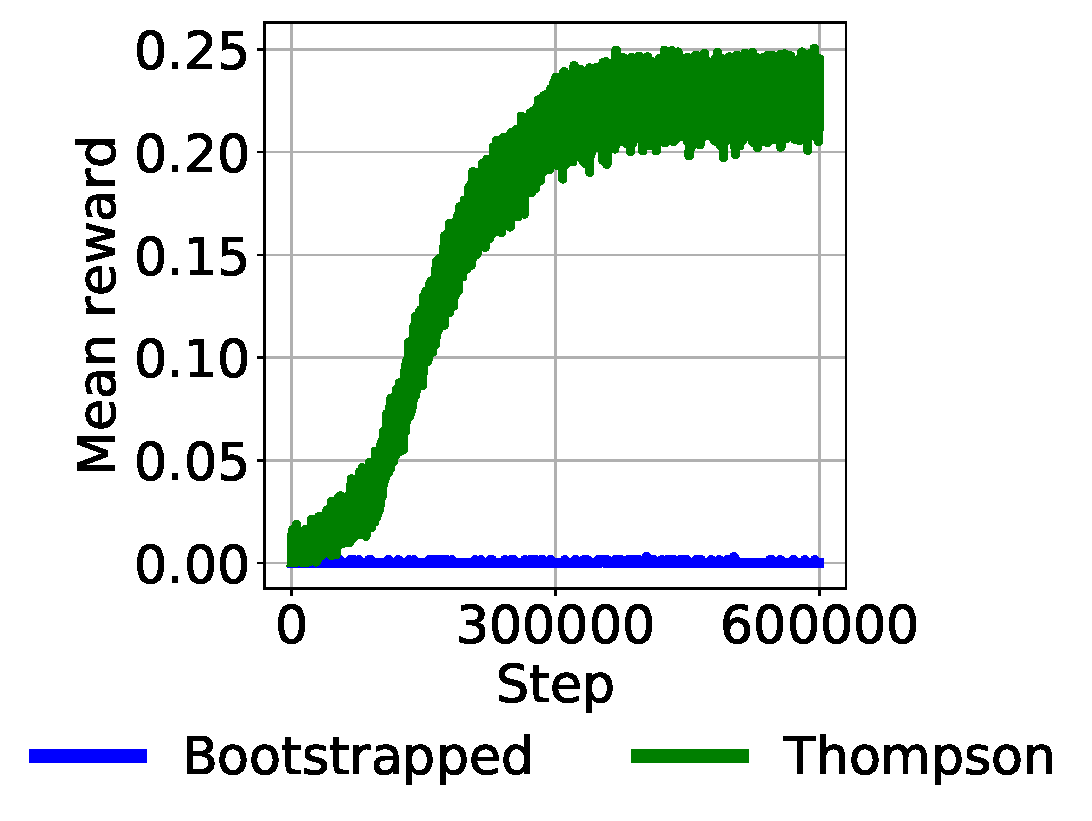
\includegraphics[scale=.25]{img/taxi_boot.pdf}}
\end{center}
\end{minipage}
\caption[Taxi problem results]{Results on the \textbf{Taxi} problem. Figure~\ref{F:taxi_online} shows the performance of the online variance estimation in terms of mean reward per step. The plots on the left show results using the setting of the policies parameters that is optimal in evaluation; the ones on the right consider parameters optimal in training. An epoch corresponds to $1000$ training steps. Figure~\ref{F:taxi_grid} shows the structure of the grid where S is the initial position of the agent, P is a passenger and G is the goal. Figure~\ref{F:taxi_boot} shows the performance during training of the bootstrapping approach in terms of mean reward per step.}\label{F:taxi}
\end{figure}
\begin{figure}[t]
\begin{minipage}{\textwidth}
\begin{center}
  \includegraphics[scale=.05]{img/bounds.pdf}
\end{center}
\end{minipage}
\caption[Taxi with different upper bounds results - 1]{Results of TS on Taxi with different upper bounds on variance.}\label{F:bounds}
\end{figure}
\begin{figure}[t]
\begin{minipage}{\textwidth}
\begin{center}
  \includegraphics[scale=.05]{img/cs.pdf}
\end{center}
\end{minipage}
\caption[Taxi with different upper bounds results - 2]{Results of TS on Taxi using Hoeffding upper bound with different values of the $c$ parameter.}\label{F:cs}
\end{figure}
\begin{figure}[t]
\begin{minipage}{\textwidth}
\begin{center}
  \includegraphics[scale=.05]{img/chics.pdf}
\end{center}
\end{minipage}
\caption[Taxi with different upper bounds results - 3]{Results of TS on Taxi using Hoeffding upper bound with $c=2$ without and with $\chi^2$ upper bound boost.}\label{F:chics}
\end{figure}
\begin{figure}[t]
\begin{minipage}{\textwidth}
\begin{center}
  \subfigure[Mountain Car\label{F:mountain_car}]{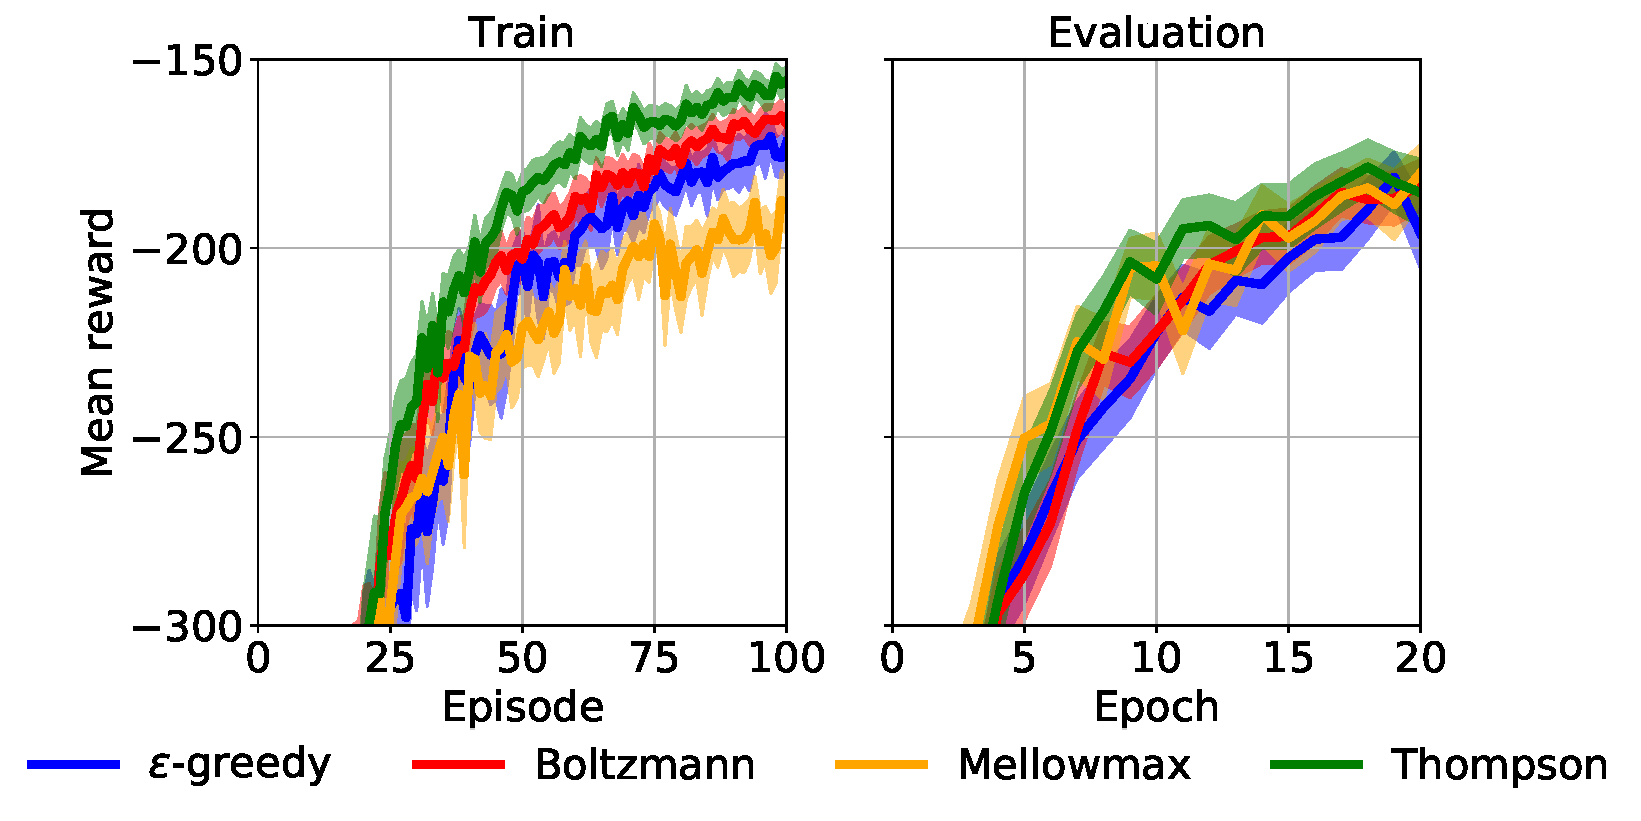
\includegraphics[scale=.3]{img/mc_comp.pdf}}
  \subfigure[Acrobot\label{F:acrobot}]{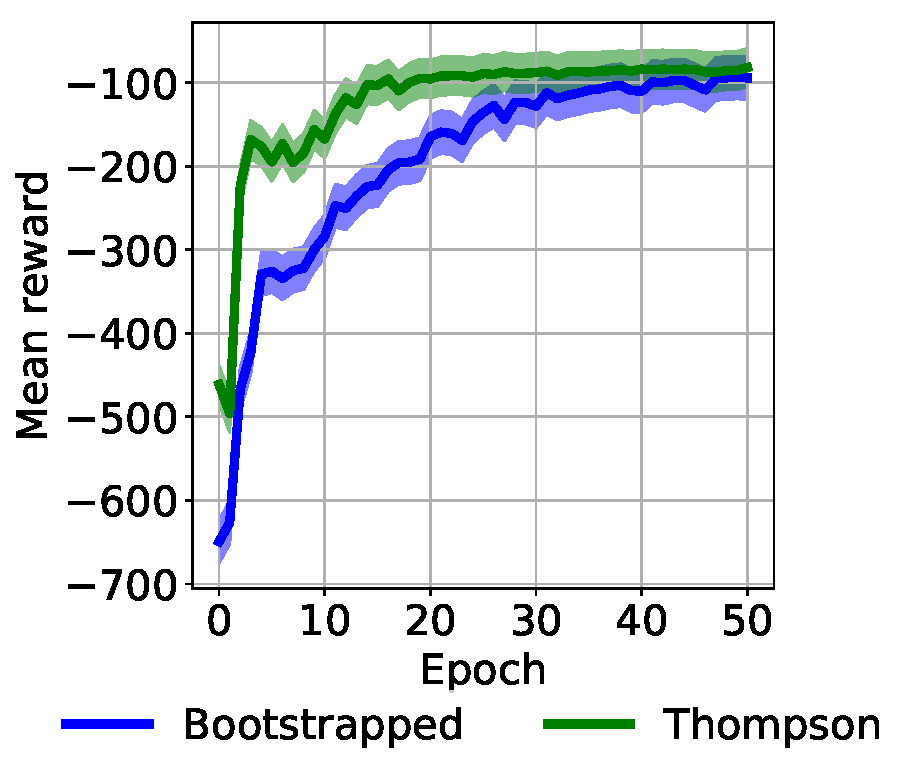
\includegraphics[scale=.3]{img/acrobot_ts.pdf}}
\end{center}
\end{minipage}
\caption[Mountain car and acrobot problems results]{Figure~\ref{F:mountain_car} shows the mean cumulative reward in train and evaluation for Mountain Car, while Figure~\ref{F:acrobot} shows the mean cumulative reward in evaluation for Acrobot. Evaluation epochs are performed every $20$ training episodes for the former, and every $1000$ training steps for the latter.}\label{F:TS_cont}
\end{figure}
\begin{figure}[t]
\begin{minipage}{\textwidth}
\begin{center}
  \subfigure[Pong\label{F:pong}]{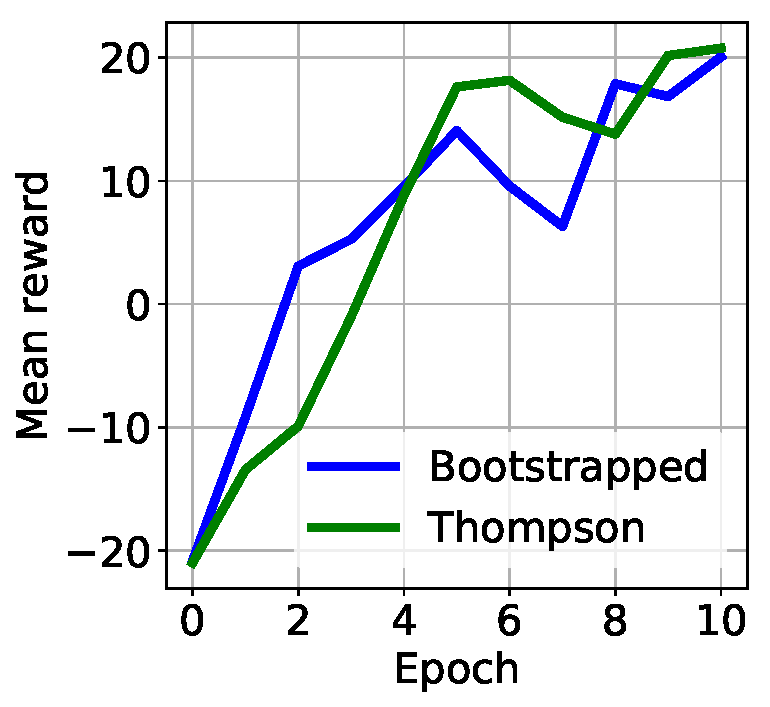
\includegraphics[scale=.3]{img/pong.pdf}}
  \hspace{1cm}
  \subfigure[Breakout\label{F:breakout}]{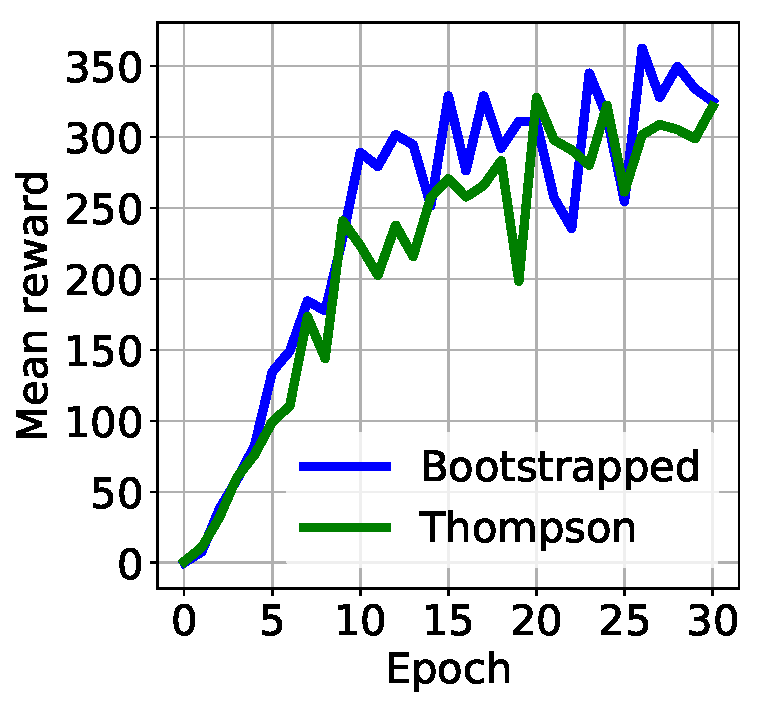
\includegraphics[scale=.3]{img/breakout.pdf}}
\end{center}
\end{minipage}
\caption[Pong and Breakout problems results]{Mean cumulative reward in evaluation. An epoch is performed every $250000$ steps.}\label{F:atari}
\end{figure}

\section{Experiments}
Our focus on the empirical evaluation of \gls{ts} over other exploration strategies is twofold since we want to show how \gls{ts} can improve and/or stabilize learning in \glspl{mdp} where exploration is a key issue, but we want also to evince how it can robustly deal with generic \glspl{mdp}.
\subsection{Discrete state space}
\subsubsection{Taxi}
\paragraph{Details} The \textbf{Taxi} problem consists of a discrete \gls{mdp}, similar to a grid world, where the agent has to collect passengers before going to the goal position. The need for exploration is intuitively critical in this problem considering the unknown location of the passengers and the sparse reward function. In particular, the balancing between exploitation-exploration is essential to avoid both suboptimal exploitive policies and slow exploratory policies. We use this problem as a small, but significant, experiment to evaluate both the online variance estimation and the bootstrapped method. We use the same configuration of the Taxi problem described in~\cite{pmlr-v70-asadi17a}. The Taxi grid is shown in Figure~\ref{F:taxi_grid} where S is the initial position of the agent, P is a passenger and G is the goal position. The actions are four: \textit{north}, \textit{south}, \textit{west} and \textit{east}. There is a probability of $0.1$ that an action fails, in this case the agent moves to one of the perpendicular directions w.r.t. the one selected. An action moving the agent towards a wall, results in no actions. The reward is always $0$, except when stepping into the goal position where it depends on the number of collected passengers: $0$ for zero, $1$ for one, $3$ for two and $15$ for three passengers. Since not only the number of passengers matters, but also which passengers have been collected, there are $264$ states in this problem. The discount factor is $\gamma = 0.99$.
\paragraph{Setting} For the results on the left of Figure~\ref{F:taxi_online}, we use $\varepsilon = 0.3$ for $\varepsilon$-greedy, temperature $\beta = 0.5$ for Boltzmann and $\omega = 1.15$ for mellowmax; the ones on the right are obtained with $\varepsilon = 0.3$ for $\varepsilon$-greedy, temperature $\beta = 1.15$ for Boltzmann and $\omega = 4.5$ for mellowmax. The learning rate is $\alpha = \frac{1}{n(s,a)^{0.3}}$ where $n(s,a)$ is the number of updates of the action value of action $a$ in state $s$. An evaluation run consists of $200$ steps. We average the results over $64$ different seeds.

The results on bootstrapping, shown in Figure~\ref{F:taxi_boot}, are obtained using $\varepsilon = 0$, learning rate $\alpha = \frac{1}{n(s,a)^{0.3}}$ and $10$ tabular approximators to do bootstrapping. The action value functions are initialized sampling from a normal distribution $\mathcal{N}(0, 1)$. The boostrapping mask is set to $1$ for all approximators. Results are averaged, and slightly smoothed, over $100$ different seeds.

We also conduct further studies on the performance of the different algorithms described in Section~\ref{S:uncertainty}. Firstly, Figure~\ref{F:bounds} shows how the upper bounds to the variance can help learning and also how $\chi^2$ upper bound with boost learns the optimal policy faster. In Figure~\ref{F:cs} is shown how the standard Hoeffding bound is able to learn the optimal policy but, as discussed in Section~\ref{S:uncertainty}, it delays too much the exploitation phase. It is also highlighted how parameter $c$ can be useful to speedup the learning, provided that it is set to a sufficiently high value in order to avoid suboptimal performance. Eventually, in Figure~\ref{F:chics} we show the improvement given by the $\chi^2$ upper bound to the Hoeffding bound with $c = 2$.
\paragraph{Results}For the online case, we compare the performance of $\chi^2$ upper bound with boost against the classic exploration strategies $\varepsilon$-greedy and Boltzmann, together with a recently proposed variant of the Boltzmann called mellowmax~\cite{pmlr-v70-asadi17a}. For the bootstrapped case, we consider tabular approximation and Double Q-Learning as the learning algorithm, opposed to \gls{bdqn}  which instead uses a deep neural network and Deep Double Q-Learning~\cite{van2016deep}; thus, we refer to this approach as \textit{Bootstrapped Q-Learning}. Figure~\ref{F:taxi_online} shows that \gls{ts} reaches better results in less time w.r.t. the other strategies. In particular, it shows how $\varepsilon$-greedy is completely ineffective in this problem, while Boltzmann and mellowmax are able to learn good policies, but still more slowly than \gls{ts}. Thus, we can conclude that here \gls{ts} shows the best balancing between exploration and exploitation. Figure~\ref{F:taxi_boot} shows similar results where surprisingly Bootstrapped Q-Learning is not able to move properly in the grid getting stuck against walls very often, while \gls{ts} manages to move in the grid by learning a good policy even if not good as in the online variance case.

\subsection{Continuous state space}
\subsubsection{Mountain Car}
\paragraph{Details} We use the \textit{MountainCar-v0} implementation available in OpenAI Gym~\cite{gym}. In this problem a car has to climb up a hill in front of it to reach a flag, but its engine is not powerful enough to climb it starting from the initial position of the car. Therefore, the car has to gain speed from the steep road behind it in order to reach the goal. The state is $2$-dimensional representing position and velocity of the car. There are $3$ actions: \textit{push left}, \textit{no push} and \textit{push right}. The reward is $-1$ at each step. The episode ends when the car reaches the flag up on the hill. The discount factor is $\gamma = 0.99$.
\paragraph{Setting} For the results in Figure~\ref{F:mountain_car}, we use the parameter settings that perform the best in training: $\varepsilon = 0.01$ for $\varepsilon$-greedy, temperature $\beta = 10.5$ for Boltzmann and $\omega = 7.5$ for mellowmax. We sparsely encode the state space with $10$ tilings of $10 \times 10$ tiles and approximate the action value function with linear approximation with weights initialized uniformly random between $-10$ and $10$. The learning rate is $\alpha = 0.1$. An evaluation epoch consists in averaging the cumulative reward per episode obtained in $5$ episodes.

\subsubsection{Acrobot}
\paragraph{Details} We use the \textit{Acrobot-v1} implementation available in OpenAI Gym~\cite{gym}. This problem consists of a pendulum with two links where only one of them is actuated. The goal is to swing the link that is the furthest to the fulcrum in such a way that it arrives to an height that has at least the length of the link closest to the fulcrum. The state is $6$-dimensional representing trigonometric measures of the pendulum. There are $3$ discrete actions to apply a torque of $-1$, $0$ or $1$ on the joint between the pendulum links. The reward is $-1$ at each step except for the step going into the goal state which returns $0$ and terminates the episode. The discount factor is $\gamma = 0.99$. 
\paragraph{Setting} For the results in Figure~\ref{F:acrobot}, we use a replay memory of $5000$ samples initialized with $100$ randomly collected samples. We use a neural network with $10$ heads composed of $2$ layers of $80$ ReLu units and a linear output unit for each action value. We optimize using Adam optimizer with learning rate $0.0001$. The batch size is $100$ and mask $m_k = 1$. The target network is updated every $100$ weight updates and the training is stopped after $50000$ steps. An evaluation epoch consists in averaging the cumulative reward per episode obtained moving for $1000$ steps.

\paragraph{Results} The need for exploration in the previously described two problems is given by the sparse reward function, even if exploration is not highly critical as in the Taxi problem. Nevertheless, we want to consider these problems to show how \gls{ts} is robust w.r.t. generic \gls{rl} problems. Since Mountain Car has a small continuous state space, we test our online variance estimation with SARSA (Algorithm~\ref{A:SARSA-apprx}) for the continuous case in this problem, while we consider the more complex Acrobot for bootstrapping. Figure~\ref{F:TS_cont} shows how \gls{ts} reaches better performance than the others and how exploration with \gls{ts} can help to speed up the convergence of the algorithm. In particular, Figure~\ref{F:mountain_car} highlights the effectiveness of exploration driven by \gls{ts} during the training phase.

\subsection{Deep Reinforcement Learning}
\paragraph{Details} We use the \textit{PongNoFrameskip-v4} and \textit{BreakoutNoFrameskip-v4} implementations of \textbf{Pong} and \textbf{Breakout} available in OpenAI Gym~\cite{gym}. The state is represented by $210 \times 160$ raw pixel frames and there are $4$ discrete actions in both of them. The reward function is sparse. In Pong, the episode ends when the score of one of the players reaches $21$. In Breakout, the episode ends when the player finishes its lives.
\paragraph{Setting} We use the same setting described in~\cite{osband2017deep}. However, in this work, it is not clear whether $\varepsilon = 0$ for Bootstrapped DQN or not. For the purpose of our work, we decide to use $\varepsilon = 0$.
\paragraph{Results} We evaluate \gls{ts} via bootstrapping in \gls{drl} considering the \textbf{Atari} games~\cite{bellemare13arcade} of \textbf{Pong} and \textbf{Breakout}. 
We have not been able to try a broader set of games for time issues; therefore we preferred quality over quantity evaluating only these two games, that can be learned faster than others, with $3$ different seeds for both. Figure~\ref{F:atari} shows that in these games \gls{ts} does not give improvements w.r.t. the \gls{bdqn} policy. However, the small number of experiments we used to average the results, the need of a better hyper-parameters search for \gls{ts} which is likely to need different settings than the one used in \gls{bdqn} and the not high relevance of exploratory actions in these two simple games, make these experiments just a preliminary evaluation of \gls{ts} in the Atari domain.
